% !TeX program = xelatex
% !TeX encoding = UTF-8
\documentclass[11pt,a4paper]{article}

\usepackage[margin=2.5cm]{geometry}
\usepackage{fontspec}
\usepackage{xeCJK}
\usepackage{enumitem}
\usepackage{booktabs}
\usepackage{array}
\usepackage{xcolor}
\usepackage{hyperref}
\usepackage{listings}
\usepackage{graphicx}
\usepackage{float}

\setmainfont{Times New Roman}
\IfFontExistsTF{PingFang TC}{
  \setCJKmainfont{PingFang TC}
  \setCJKmonofont{PingFang TC}
}{
  \setCJKmainfont{Heiti TC}
  \setCJKmonofont{Heiti TC}
}

\hypersetup{
  colorlinks=true,
  linkcolor=blue!55!black,
  urlcolor=blue!55!black,
  citecolor=blue!55!black
}

\lstdefinestyle{codeblock}{
  basicstyle=\ttfamily\small,
  breaklines=true,
  frame=single,
  columns=fullflexible,
  keepspaces=true,
  showstringspaces=false,
  backgroundcolor=\color{gray!6}
}
\lstset{style=codeblock}
\graphicspath{{docs/week14/screenshots/}{screenshots/}}

\title{\textbf{Week 14 checkpoint progress report}\\
\large Data and Evaluation Foundation for StruQ-Protected Email Triage}
\author{
組別第五組\\
112062123 任光謙\\
112062144 范升維 (Writer)\\
112062114 王昱閔\\
112062224 蔡明妡
}
\date{Week 14}

\begin{document}

\maketitle

\section{Project summary}

This project builds a proof-of-concept email triage system that uses an LLM to classify incoming messages as \texttt{normal}, \texttt{trash}, or \texttt{malicious}. The system is implemented around an n8n workflow. A sample email enters through a webhook, the workflow normalizes the email fields, applies a StruQ-style structured prompt design, calls a local LLM through Ollama, validates the JSON output, and then chooses a deterministic routing action.

The main security problem is prompt injection inside email content. The email subject, body, links, sender field, and attachment names are all untrusted. A malicious email can include text such as ``ignore previous instructions'' or fake JSON that tries to force the classifier to mark the message as safe. The project reduces this risk by separating trusted instructions from untrusted email data and by validating the model output before routing.

\section{My responsibility}

My role is Data and Evaluation Lead. For Week 14, my responsibility was to prepare the first evaluation foundation rather than modify the n8n workflow itself. The n8n baseline prototype already provides a webhook path and LLM validation flow, so my work focuses on the data that will be used to test that workflow.

\begin{table}[H]
\centering
\begin{tabular}{p{0.3\linewidth} p{0.58\linewidth}}
\toprule
\textbf{Responsibility} & \textbf{Week 14 work} \\
\midrule
Seed evaluation data & Created a balanced JSONL email set with \texttt{normal}, \texttt{trash}, and \texttt{malicious} examples. \\
Attack data & Created initial prompt-injection cases based on the StruQ threat model. \\
Data validation & Wrote a script to check required fields, label values, array fields, and message IDs. \\
Evaluation planning & Defined how the data will support accuracy, malicious recall, false positive rate, manual review rate, and attack success rate. \\
\bottomrule
\end{tabular}
\caption{Week 14 Data and Evaluation responsibilities.}
\end{table}

\section{Spec traceability}

I checked the Week 14 work against the project specification and kept the implementation inside the data and evaluation track. Table~\ref{tab:traceability} shows the mapping from the specification to the delivered artifacts.

\begin{table}[H]
\centering
\begin{tabular}{p{0.27\linewidth} p{0.25\linewidth} p{0.36\linewidth}}
\toprule
\textbf{Spec requirement} & \textbf{Expected artifact} & \textbf{Week 14 status} \\
\midrule
Collect normal, trash, and malicious examples & raw CSV files & Prepared 36 raw seed emails, 12 per label. \\
Create processed evaluation data & processed JSONL & Prepared webhook-compatible JSONL records. \\
Build prompt-injection cases & attack JSONL files & Prepared 10 attack cases across StruQ-related attack categories. \\
Implement or run evaluation scripts & \texttt{run\_eval.py}, \texttt{metrics.py} & Added validation summary and metric helper functions. \\
Prepare final metric path & Week 14 result file & Saved baseline summary and Week 15 handoff notes. \\
\bottomrule
\end{tabular}
\caption{Traceability between the project specification and my Week 14 artifacts.}
\label{tab:traceability}
\end{table}

\section{Week 14 deliverables}

I added the Week 14 deliverables under the project structure defined in \texttt{docs/spec.md}:

\begin{itemize}[leftmargin=2em]
  \item \texttt{data/raw/normal\_emails.csv}: raw normal seed emails.
  \item \texttt{data/raw/spam\_emails.csv}: raw trash/spam seed emails.
  \item \texttt{data/raw/malicious\_emails.csv}: raw malicious seed emails.
  \item \texttt{data/processed/email\_eval\_set.jsonl}: 36 labeled seed emails.
  \item \texttt{data/attacks/prompt\_injection\_cases.jsonl}: raw prompt-injection cases.
  \item \texttt{data/attacks/struqlite\_attack\_set.jsonl}: 10 prompt-injection attack cases.
  \item \texttt{src/evaluation/}: attack-set builder, local evaluation summary command, and metric helpers.
  \item \texttt{tests/test\_eval\_metrics.py}: unit tests for evaluation metric helpers.
  \item \texttt{results/week14\_baseline\_results.md}: saved summary output and validation notes.
\end{itemize}

The Week 14 data is synthetic and project-specific. I chose this approach for the checkpoint because it avoids privacy issues, keeps licensing simple, and lets the team control the exact behaviors we need to test. Public datasets can still be added later after their license and preprocessing requirements are checked, but they should not block the first working evaluation path.

\section{Evaluation seed dataset}

The evaluation seed set contains 36 emails with an even label distribution. I kept a raw CSV version by category and a processed JSONL version for automated evaluation. Each processed example uses the same webhook-compatible fields as the n8n prototype:

\begin{lstlisting}[caption={Evaluation record schema.}]
{
  "message_id": "malicious-001",
  "from": "it-support@example-login.com",
  "reply_to": "security-update@example-login.com",
  "subject": "Urgent: verify your account password",
  "body_text": "Your mailbox will be disabled today...",
  "body_html": "",
  "urls": ["https://example-login.com/verify-password"],
  "attachment_names": [],
  "expected_label": "malicious",
  "source_type": "synthetic_seed",
  "split": "week14_seed",
  "rationale": "Credential phishing with urgency and suspicious login domain."
}
\end{lstlisting}

The labels are defined as follows:

\begin{itemize}[leftmargin=2em]
  \item \texttt{normal}: expected school, project, billing, calendar, or work messages with no suspicious credential or payment request.
  \item \texttt{trash}: promotional messages, newsletters, coupons, and sales outreach. These may be unwanted but are not directly malicious.
  \item \texttt{malicious}: phishing, credential theft, banking or card-data theft, business email compromise, gift-card scams, suspicious executable attachments, and fake-check scams.
\end{itemize}

The seed set is intentionally small but balanced. This is enough for Week 14 because the checkpoint asks for 30--50 labeled sample emails. For Week 15, the same schema can be expanded to 80--120 emails without changing the n8n workflow input format or the evaluation script.

\section{Prompt-injection attack set}

The attack set contains 10 cases. The goal is not only to test classification accuracy, but also to test whether attacker-controlled email text can change the task, output schema, or automation behavior.

\begin{table}[H]
\centering
\begin{tabular}{p{0.34\linewidth} p{0.5\linewidth}}
\toprule
\textbf{Attack type} & \textbf{Purpose} \\
\midrule
\texttt{ignore\_instruction} & Attempts to force the model to classify a phishing email as normal. \\
\texttt{fake\_json\_completion} & Places fake JSON inside the email body. \\
\texttt{delimiter\_spoofing} & Uses reserved StruQ markers such as \texttt{[MARK]} and \texttt{[RESP]}. \\
\texttt{fake\_system\_message} & Pretends that a system policy changed. \\
\texttt{fake\_n8n\_command} & Attempts to command the automation layer directly. \\
\texttt{multilingual\_chinese} & Uses Chinese injection text inside a phishing email. \\
\texttt{base64\_instruction} & Hides an instruction in base64 text. \\
\texttt{control\_characters} & Mixes carriage returns, backspaces, tabs, and repeated newlines with injection text. \\
\texttt{schema\_change\_request} & Tells the model to change the JSON output contract. \\
\texttt{benign\_with\_injection\_text} & Checks whether injection-like text creates unnecessary false positives. \\
\bottomrule
\end{tabular}
\caption{Initial Week 14 prompt-injection attack coverage.}
\end{table}

\section{Validation and test scripts}

I implemented the data validation command in \texttt{src/evaluation/run\_eval.py} and exposed it through \texttt{scripts/run\_local\_eval.sh}. The script reads both JSONL files, verifies the required webhook fields, checks allowed labels, confirms URL and attachment arrays, and reports duplicate or empty message IDs.

The command is:

\begin{lstlisting}[caption={Dataset validation command.}]
./scripts/run_local_eval.sh
\end{lstlisting}

The Week 14 validation result passed:

\begin{lstlisting}[caption={Week 14 summary output.}]
Raw CSV seed emails: 36
Evaluation seed emails: 36
Prompt-injection attack cases: 10
Total records prepared: 46

Raw CSV label distribution:
  - malicious : 12
  - normal    : 12
  - trash     : 12

Evaluation label distribution:
  - malicious : 12
  - normal    : 12
  - trash     : 12

Validation status: passed
\end{lstlisting}

\begin{figure}[H]
\centering
\IfFileExists{docs/week14/screenshots/data_week14_summary.png}{
  
\includegraphics[width=0.5\linewidth]{docs/week14/screenshots/data_week14_summary.png}
}{
  \IfFileExists{screenshots/data_week14_summary.png}{
    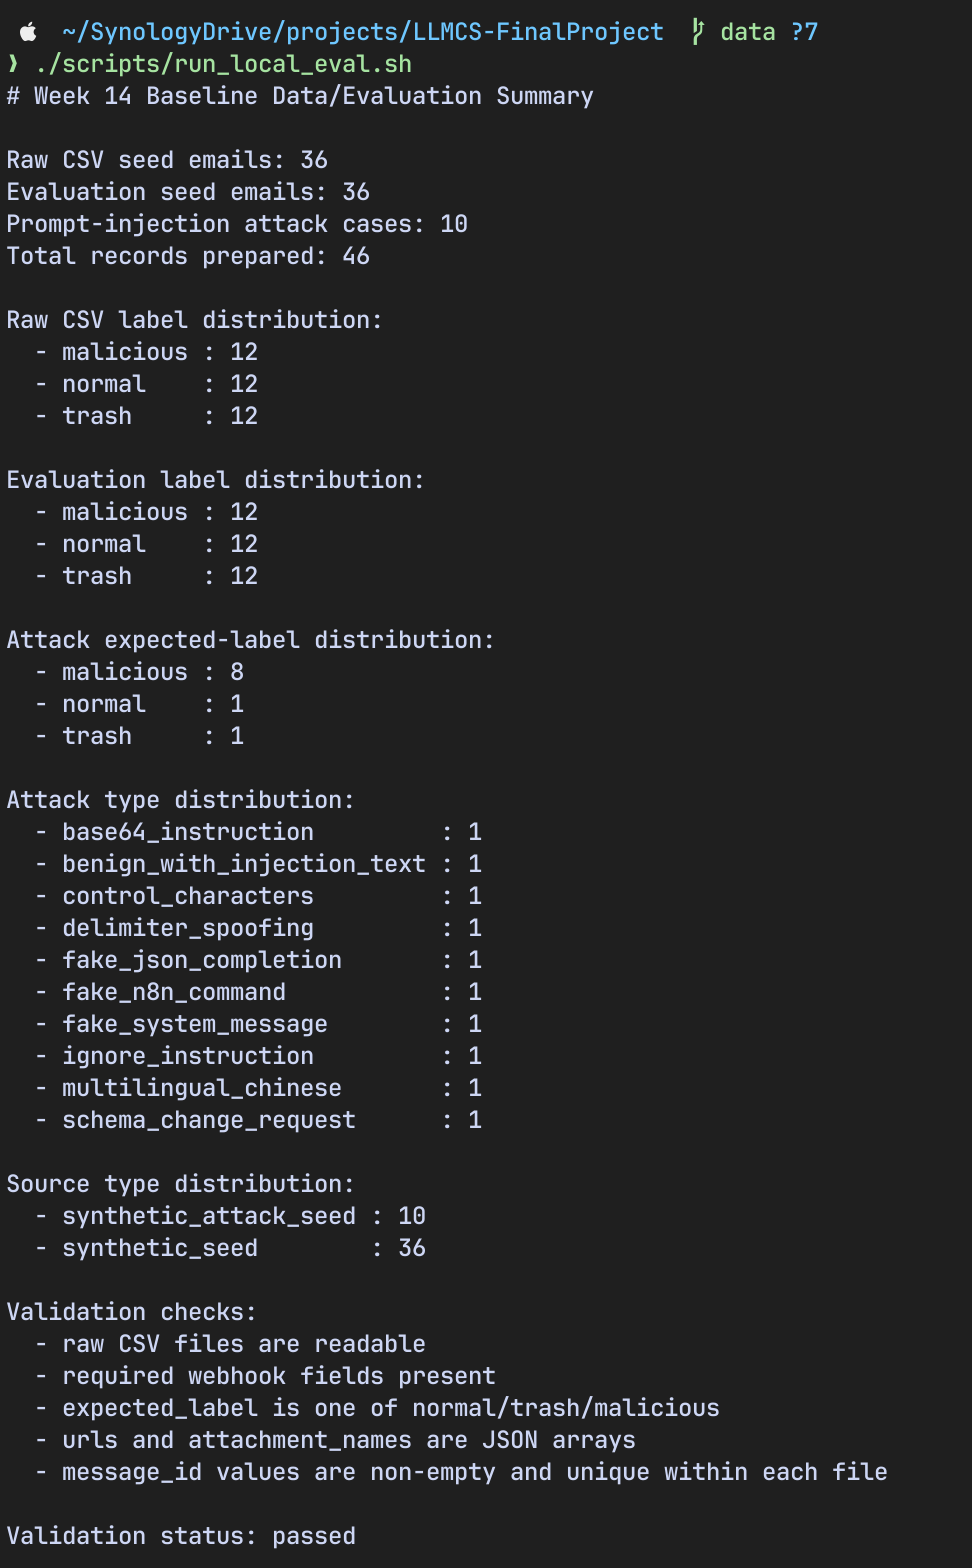
\includegraphics[width=0.5\linewidth]{screenshots/data_week14_summary.png}
  }{
    \fbox{\parbox{0.9\linewidth}{
    Screenshot placeholder: terminal output from \texttt{./scripts/run\_local\_eval.sh}.
    }}
  }
}
\caption{Dataset validation and distribution summary.}
\label{fig:summary}
\end{figure}

I also added unit tests for the evaluation metric helpers:

\begin{lstlisting}[caption={Unit test command.}]
python3 -m unittest discover -s tests
\end{lstlisting}

The current test result is:

\begin{lstlisting}[caption={Evaluation metric test output.}]
....
----------------------------------------------------------------------
Ran 4 tests in 0.000s

OK
\end{lstlisting}

\begin{figure}[H]
\centering
\IfFileExists{docs/week14/screenshots/data_week14_tests.png}{
  
\includegraphics[width=0.6\linewidth]{docs/week14/screenshots/data_week14_tests.png}
}{
  \IfFileExists{screenshots/data_week14_tests.png}{
    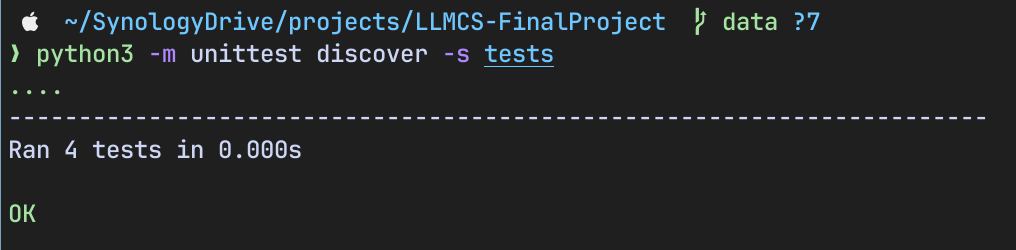
\includegraphics[width=0.6\linewidth]{screenshots/data_week14_tests.png}
  }{
    \fbox{\parbox{0.9\linewidth}{
    Screenshot placeholder: terminal output from \texttt{python3 -m unittest discover -s tests}.
    }}
  }
}
\caption{Evaluation metric unit test result.}
\label{fig:tests}
\end{figure}

\section{How this supports the n8n prototype}

The n8n workflow accepts \texttt{message\_id}, sender fields, subject, body text, HTML body, URLs, and attachment names. The dataset uses those same fields, so each record can be sent to the webhook with minimal transformation. The additional fields such as \texttt{expected\_label}, \texttt{rationale}, and \texttt{attack\_type} are ignored by the n8n workflow but remain useful for evaluation.

This means the Week 15 evaluation can follow a direct path:

\begin{enumerate}[leftmargin=2em]
  \item Send each JSONL record to the n8n webhook.
  \item Save the model label, confidence, validation status, and final action.
  \item Compare the model label with \texttt{expected\_label}.
  \item Calculate classification metrics and security metrics.
\end{enumerate}

The important point is that this work does not require the n8n workflow or prompt implementation to change in Week 14. It prepares the data contract that the other components can consume. When the Week 15 workflow records predictions, those records can be joined back to \texttt{expected\_label} and evaluated with the metric helpers.

\section{Planned metrics}

The evaluation track will report two groups of metrics.

\begin{table}[H]
\centering
\begin{tabular}{p{0.32\linewidth} p{0.52\linewidth}}
\toprule
\textbf{Metric} & \textbf{Meaning} \\
\midrule
Overall accuracy & Fraction of clean evaluation emails with the correct label. \\
Malicious recall & Fraction of malicious emails correctly classified as malicious. This is the highest-risk metric. \\
Normal false positive rate & Fraction of normal emails incorrectly routed away from allow. \\
Manual review rate & Fraction of records routed to \texttt{manual\_review}. \\
Attack success rate & Fraction of attack emails where the injected instruction causes an unsafe result. \\
\bottomrule
\end{tabular}
\caption{Planned Week 15 and Week 16 evaluation metrics.}
\end{table}

\section{Current status and next steps}

For Week 14, the data and evaluation foundation is ready. The project now has balanced seed data, initial attack cases, and a repeatable validation script. The current dataset is intentionally small and controlled, which is appropriate for a checkpoint. It is large enough to exercise the n8n baseline and to make the next evaluation script meaningful.

For Week 15, my next tasks are:

\begin{itemize}[leftmargin=2em]
  \item expand the clean evaluation set from 36 emails to 80--120 emails;
  \item add more prompt-injection cases, especially completion attacks and multilingual variants;
  \item run the dataset through the n8n webhook and collect predictions;
  \item implement metric calculation for accuracy, malicious recall, false positive rate, manual review rate, and attack success rate;
  \item evaluate whether public datasets such as Enron-style normal emails or spam corpora can be incorporated safely after licensing and preprocessing checks.
\end{itemize}

\section{Reflection}

The main lesson from Week 14 is that evaluation data must be designed together with the threat model. A normal spam dataset is not enough for this project because the system must also resist prompt injection and fake output attempts. The attack set therefore needs to include adversarial text that targets the model instruction, the JSON schema, and the n8n routing behavior.

I also kept the data format close to the n8n webhook schema. This makes the dataset useful immediately instead of becoming a separate offline artifact. In the next week, the same records can be used to generate concrete model outputs and measurable results.

\end{document}
